\begin{figure*}[t]
\centering
\begin{minipage}{0.47\textwidth}
    \centering
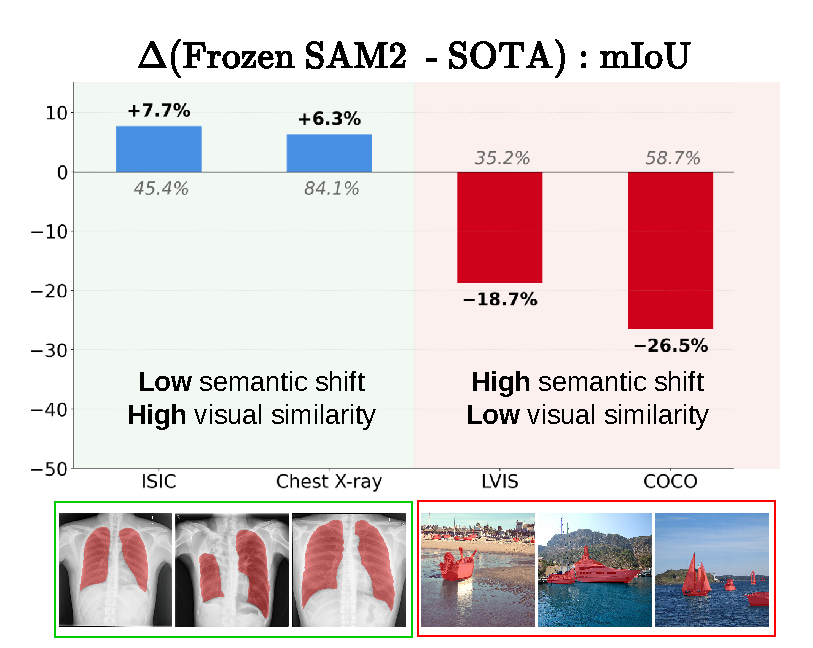
\includegraphics[width=\textwidth]{images/teaser1.pdf}
    \caption{We evaluate frozen \sam{} on few-shot segmentation tasks on four datasets with varying degrees of semantic variability. On datasets \cite{candemir2013lung, codella2019skin} with low semantic shift and high intra-class visual similarity, SAM2 matches or even outperforms state-of-the-art APSeg~\cite{he2024apseg}. However, on more challenging datasets like COCO and LVIS, with high semantic shift (\eg, \textit{cruise ship} vs. \textit{rowboat}), its performance drops significantly, compared with GF-SAM \cite{zhang2024bridge}. The bottom row illustrates examples of ground-truth masks in both scenarios.}
    \label{fig:isic}
\end{minipage}
\hspace{6pt}
\begin{minipage}{0.47\textwidth}
    \centering
    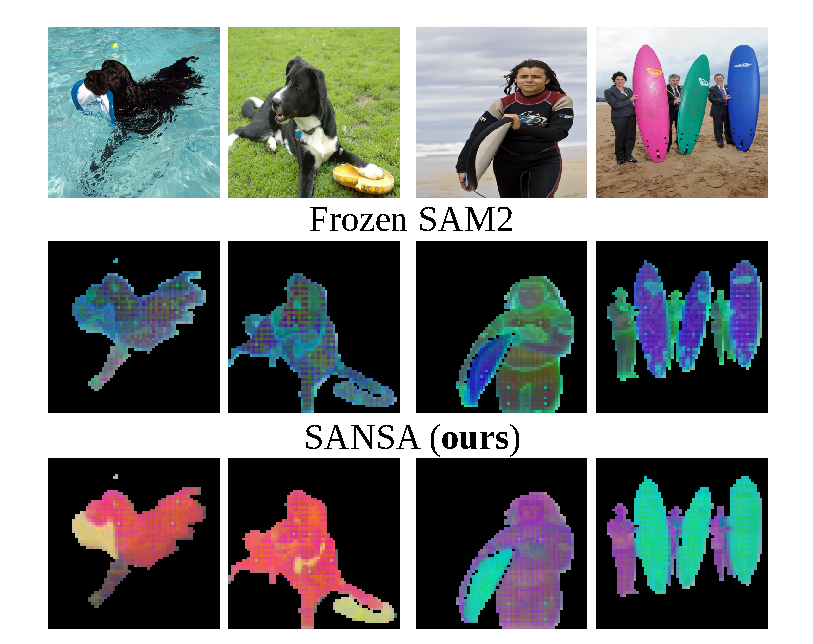
\includegraphics[width=\textwidth]{images/teaser2.pdf}
    %\vspace{0.1cm}
    \caption{We extract \sam{} features from object instances across diverse images and visualize their distribution using the first three principal components of PCA, mapped to RGB channels. The features appear entangled, with clusters mixing across categories, highlighting the lack of a coherent semantic structure in the original feature space. After adapting the feature space with SANSA, well-defined clusters emerge: semantically similar instances group together, forming coherent structures despite intra-class variation in visual appearance.}
    \label{fig:teaser_feat}
\end{minipage}
\vspace{-0.6cm}
%\caption{Overall figure caption describing all three images.}
\end{figure*}